% =====================================================================
% part1_openmp.tex -- PARTE 1: Simulazione shared-memory con OpenMP
% Membro responsabile: ___________________
% Puoi modificare liberamente da qui in poi, non toccare gli altri file.
% =====================================================================
\section{Part 1 -- Shared-Memory Simulation with OpenMP}
\label{sec:openmp}

\subsection{Problem Description}
The first part of the project requires the implementation of a
sequential-to-parallel simulator of the damped wave equation
introduced in Section~1 (Eq.~1), parallelized using OpenMP. Given
the physical parameters $\gamma$ (damping) and $c$ (propagation
speed), and the numerical parameters $\Delta t$, $\Delta x$, the
grid size $M$, and the number of time steps $N$, the simulator must
compute the evolution of the wave height matrix $u^n_{i,j}$ starting
from an initial condition where the matrix is uniformly zero except
for an initial impulse applied at a boundary point $(i_0, j_0)$ at
$n=0$.

\subsection{Numerical Method and Implementation}
\label{sec:numerical-method}
At each time step, the simulator applies the explicit update rule
of Equation~(3) using a nine-point isotropic Laplacian stencil,
which requires keeping in memory the wave fields at the two
previous time steps ($u^n$ and $u^{n-1}$) to compute $u^{n+1}$.
The computation is organized as a loop over the $N-1$ frames to be
generated (the initial condition is written as frame~0 before the
loop starts); for each frame, the update is applied independently to
every interior grid point $(i,j)$, which makes the spatial loop
embarrassingly parallel and well suited to a \texttt{\#pragma omp
parallel for} directive.

\paragraph{9-point vs.\ 5-point stencil.} The standard 5-point
Laplacian is only an approximate, direction-dependent operator: its
leading truncation error is not isotropic, so a point-source wave
propagating on a coarse grid tends to acquire a visibly
non-circular (roughly diamond/square-shaped) wavefront, most
noticeable at larger radii from the source. The 9-point stencil used
here, $\nabla^2 u \approx \frac{1}{6\Delta x^2}\big[4(\text{edge
neighbours}) + (\text{diagonal neighbours}) - 20\,u\big]$, blends
axis-aligned and diagonal neighbours and is a standard choice in
finite-difference acoustic/wave modelling precisely because it
reduces this directional bias, yielding visibly more circular
wavefronts without changing the overall $O(\Delta x^2)$ accuracy of
the scheme. A von Neumann stability analysis of this operator gives
a maximum discrete eigenvalue magnitude of $16/(3\Delta x^2)$,
versus $8/\Delta x^2$ for the 5-point stencil; substituting into the standard leapfrog stability bound
$c^2\Delta t^2\lambda_{\max}\le 4$ yields, for the 9-point stencil,
\[
\frac{c\,\Delta t}{\Delta x} \le \frac{\sqrt{3}}{2} \approx 0.866,
\]
compared to the classical 5-point bound
\[
\frac{c\,\Delta t}{\Delta x} \le \frac{1}{\sqrt2} \approx 0.707.
\]
The 9-point operator is therefore, somewhat counter-intuitively,
\emph{less} restrictive than the classical 5-point CFL bound; $\Delta
x$ and $\Delta t$ (Table~1) were chosen to satisfy this
relaxed condition with margin, rather than the stricter 5-point one.

\paragraph{Frame count and playback rate.} $N$ and the output frame
rate were chosen jointly rather than independently: at $120$ fps the
$N=3840$ frames yield a $32\,\mathrm{s}$ video, long enough to show
the wavefront traverse the domain and the amplitude visibly decay
under $\gamma$, while $120$ fps comfortably exceeds the
$24$-$60$ fps range normally sufficient for perceptually smooth
motion, avoiding visible stepping on the fast-moving wavefront
immediately after the impulse.

\paragraph{Complexity.} Each time step updates $O(M^2)$ interior
points at $O(1)$ cost per point (fixed 9-neighbour stencil), giving
$O(M^2)$ work per frame and $O(NM^2)$ total sequential work over the
simulation; with $P$ OpenMP threads the compute kernel scales as
$O(NM^2/P)$ in the ideal case. Memory use is $O(M^2)$ and independent
of $N$, since only three $M\times M$ buffers (\texttt{old},
\texttt{current}, \texttt{new}) plus one color buffer are kept
resident at any time -- frames are streamed to disk incrementally
rather than accumulated in memory.

The same row-wise \texttt{\#pragma omp parallel for
schedule(static)} pattern used for the update is also applied to
initialize the fields at $n=0$ and to rescale each frame to
$[0,255]$ (Section~\ref{sec:parallelization}).

Boundary points are excluded from the update loop ($i,j \in
[1,M-2]$) and are therefore left at their initial value rather than
being explicitly reflected or clamped; since the initial Gaussian
pulse is confined well inside the domain, the border cells
effectively behave as a fixed (Dirichlet-like) zero boundary,
provided $M$ is large enough that the wavefront does not reach the
edges during the simulated interval.

After each time step, the matrix is rescaled to $[0,255]$ and
written as a P5-encoded PGM frame (\texttt{frame\_\%05d.pgm}); the
rescaling range is derived once, before the time loop, from the
pulse intensity ($[-|\text{intensity}|, +|\text{intensity}|]$)
rather than recomputed per frame, keeping the gray-level mapping
consistent across the video at the cost of clipping any point that
exceeds the assumed range. FFmpeg then assembles the frames into an
MP4 at the frame rate discussed above.

\subsection{Parallelization Strategy}
\label{sec:parallelization}
Since every interior point writes only to its own entry of
\texttt{new}, reading exclusively from the read-only \texttt{old}
and \texttt{current} arrays of the previous two time steps, the
workload is perfectly uniform and requires no synchronization within
the loop body. \texttt{schedule(static)} was therefore preferred
over dynamic scheduling: a fixed, contiguous row-wise partitioning
balances the identical per-row workload without the runtime overhead
of dynamic assignment, and preserves cache locality since each
thread's contiguous rows match the access pattern of
\texttt{wave\_update\_9\_pts}. No false sharing is expected either,
as adjacent threads' chunks are separated by a full row of $M$
elements rather than by individual cache-line-sized entries.

The number of OpenMP threads was varied over $T \in \{1, 2, 4, 8,
16, 32, 48\}$, using \texttt{OMP\_NUM\_THREADS} together with
\texttt{OMP\_PROC\_BIND=true} and \texttt{OMP\_PLACES=cores} to pin
threads to physical cores. As discussed in Section~\ref{sec:results},
profiling with Intel VTune revealed that, for the tested grid sizes,
the per-frame PGM file-writing routine
(\texttt{write\_snapshot\_serial}) -- strictly serial in the current
implementation -- accounts for a substantial fraction of wall-clock
time independently of thread count; by Amdahl's Law, this serial
I/O fraction alone places a hard ceiling on achievable speedup, which
the results below confirm empirically.

\subsection{Results}
\label{sec:results}
Simulations were run on the \texttt{cpu\_sapphire} partition of the
Legion cluster, with $M=2000$ and $N=3840$ (Table~1), sweeping
$T \in \{1,2,4,8,16,32,48\}$. Timings were measured directly via
\texttt{omp\_get\_wtime()}; Intel VTune Hotspots and Threading
collections additionally measured effective CPU utilization and the
CPU-time/Wait-time breakdown.

\subsubsection{Execution Time, Speedup and Efficiency}
Figure~2 shows execution time, speedup, and efficiency vs.\ thread
count. Time drops from $360.4\,\mathrm{s}$ at $T=1$ to
$231.2\,\mathrm{s}$ at $T=48$, but far from proportionally: speedup
saturates at $1.56\times$ (vs.\ an ideal $48\times$), and efficiency
collapses from 100\% to 3.2\% (Table~2). A non-monotonic point at
$T=8$ ($298.5\,\mathrm{s}$, slower than $T=4$'s $292.5\,\mathrm{s}$)
is consistent with scheduling/NUMA overhead occasionally outweighing
the marginal parallel gain once thread count exceeds the useful
parallel work available per frame.

\subsubsection{CPU Utilization and the I/O Bottleneck}
Effective CPU Utilization stays under 1\% for $T\le 8$ and reaches
only 5.2\% at $T=48$ -- far below what a compute-bound workload
would show. Figure~3 confirms why: CPU time grows with thread count
(from $106.9\,\mathrm{s}$ to $1220.6\,\mathrm{s}$, aggregate work
across threads), while Wait time stays essentially flat around
$47$--$48\,\mathrm{s}$ up to $T=16$ and rises only moderately at
$T=32$/$48$ ($57.9\,\mathrm{s}$/$59.0\,\mathrm{s}$). The serial
frame-writing stage is a fixed cost that thread count cannot reduce.

\subsubsection{Discussion}
The simulator is I/O-bound, not compute-bound, at this problem size:
\texttt{wave\_update\_9\_pts} scales well in isolation, but serial
frame writing caps observed speedup at $1.56\times$ instead of the
theoretical $48\times$, matching the Amdahl's Law prediction of
Section~\ref{sec:parallelization} and pointing to I/O -- e.g.\
buffered/asynchronous writing, or reduced snapshot frequency -- as
the primary target for future optimization rather than further
thread-level parallelism.

\begin{table}[h]
\centering
\caption{Simulation parameters -- Part 1.}
\label{tab:part1-params}
\begin{tabular}{ll}
\toprule
Parameter & Value \\
\midrule
$\gamma$ (damping)        & 0.152 \\
$c$ (propagation speed)   & 0.55 \\
$\Delta t$                & 0.0083 \\
$\Delta x$                & 0.025 \\
$M$ (grid size)           & 2000 \\
$N$ (number of frames)    & 3840 \\
\bottomrule
\end{tabular}
\end{table}

\begin{table}[h]
\centering
\footnotesize
\caption{Execution time, speedup, efficiency, and CPU utilization vs.\ OpenMP thread count ($M=2000$, $N=3840$).}
\label{tab:part1-scaling}
\begin{tabular}{rrrrr}
\toprule
Threads & Time (s) & Speedup & Efficiency (\%) & CPU Util.\ (\%) \\
\midrule
1  & 360.37 & 1.00 & 100.0 & 0.30 \\
2  & 348.30 & 1.04 & 51.7  & 0.40 \\
4  & 292.52 & 1.23 & 30.8  & 0.70 \\
8  & 298.50 & 1.21 & 15.1  & 0.90 \\
16 & 274.05 & 1.32 & 8.2   & 1.50 \\
32 & 239.67 & 1.50 & 4.7   & 3.70 \\
48 & 231.22 & 1.56 & 3.2   & 5.20 \\
\bottomrule
\end{tabular}
\end{table}

\begin{figure}[H]
\centering
\begin{subfigure}[b]{0.32\linewidth}
    
\includegraphics[width=\linewidth]{frames/frame_start.png}
    \caption{$t = 0$}
\end{subfigure}
\hfill
\begin{subfigure}[b]{0.32\linewidth}
    
\includegraphics[width=\linewidth]{frames/frame_mid.png}
    \caption{$t \approx N/2$}
\end{subfigure}
\hfill
\begin{subfigure}[b]{0.32\linewidth}
    
\includegraphics[width=\linewidth]{frames/frame_end.png}
    \caption{$t \approx N$}
\end{subfigure}
\caption{Example frames of the wave simulation at different time steps, showing propagation and progressive damping of the wave amplitude.}
\label{fig:part1-frames}
\end{figure}

\begin{figure}[h]
\centering
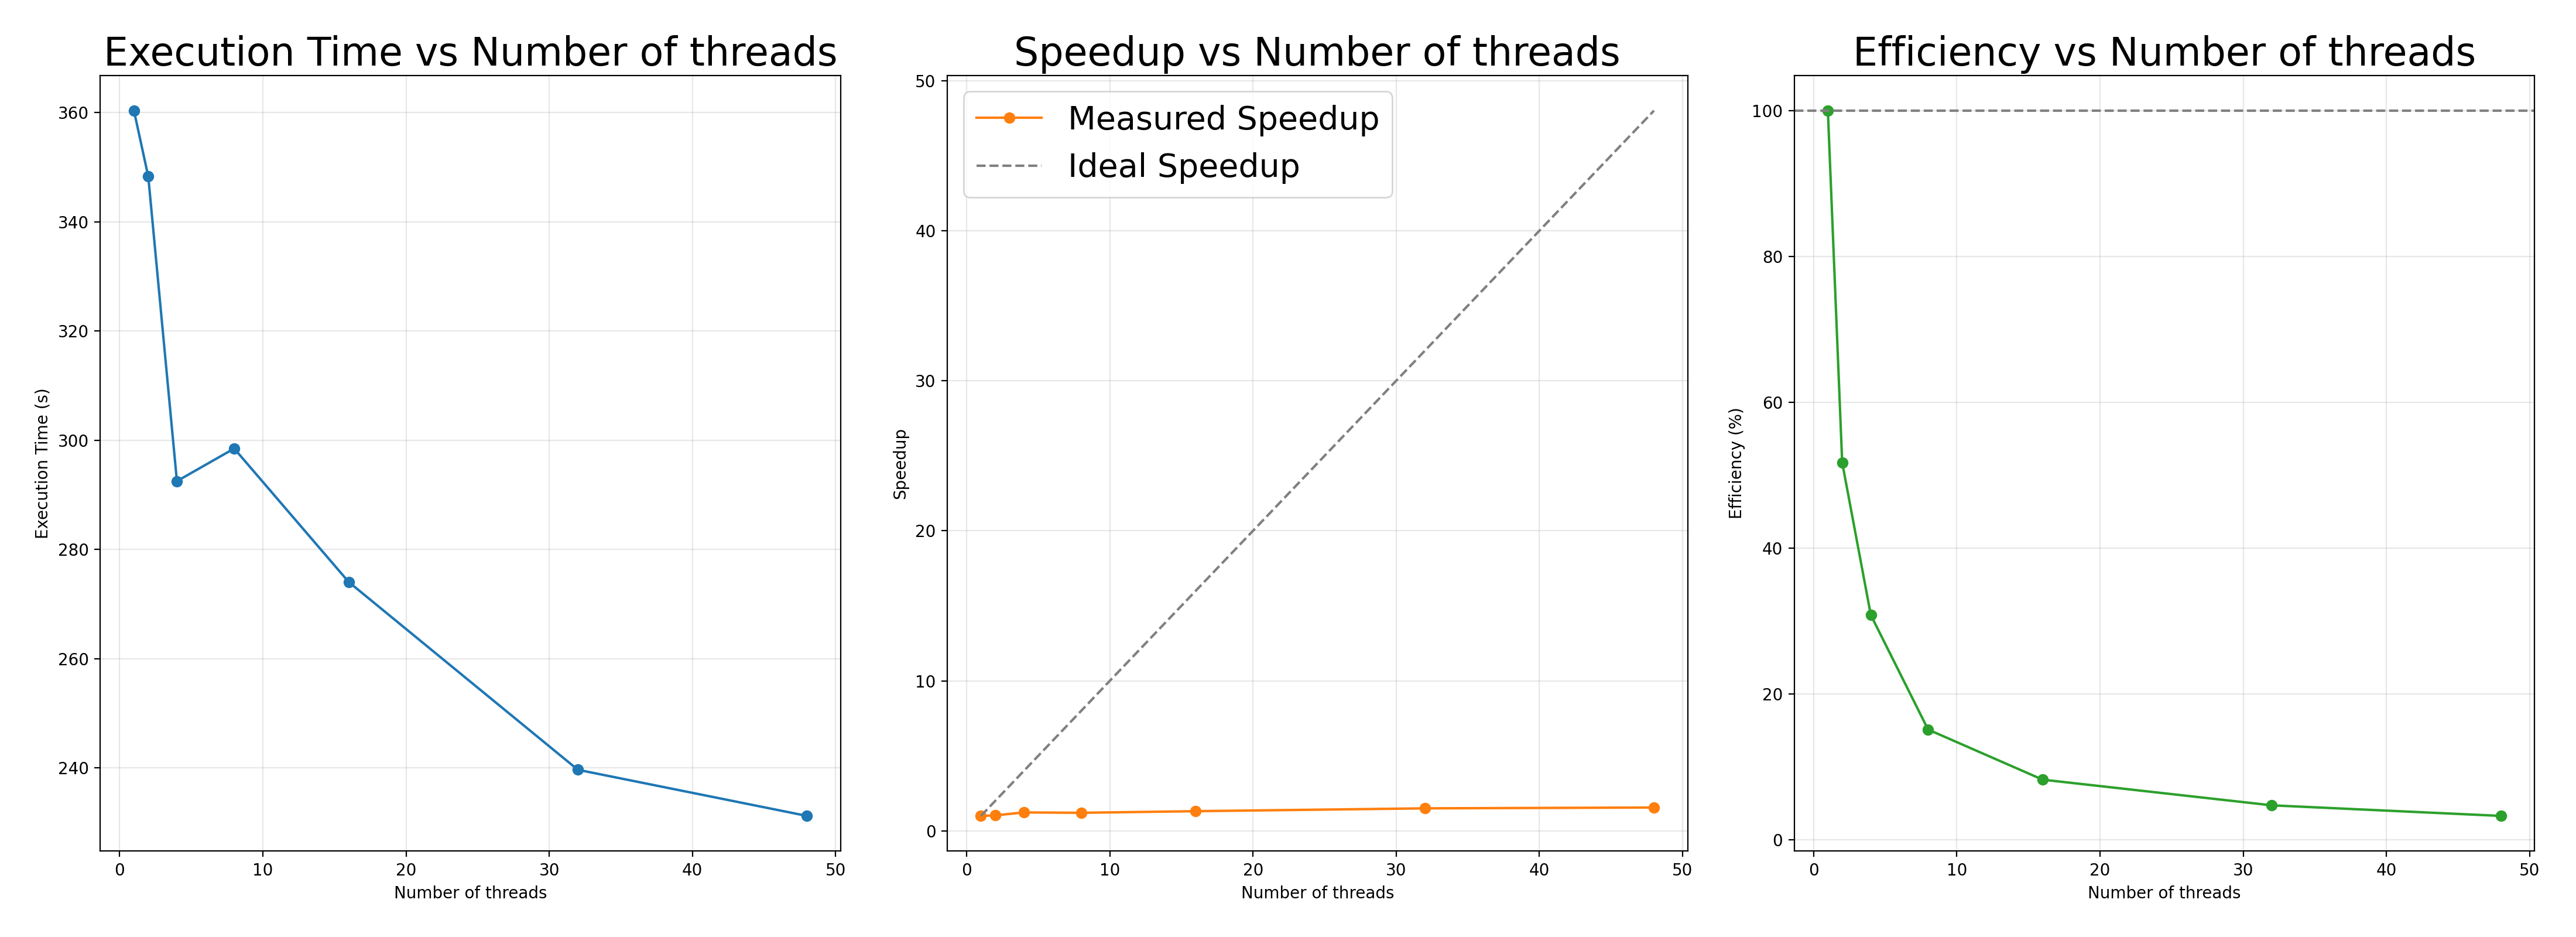
\includegraphics[width=1.0\linewidth]{scaling_plot.png}
\caption{Execution time, speedup, and parallel efficiency as a function of the number of OpenMP threads ($M=2000$, $N=3840$).}
\label{fig:part1-speedup}
\end{figure}

\begin{figure}[h]
\centering
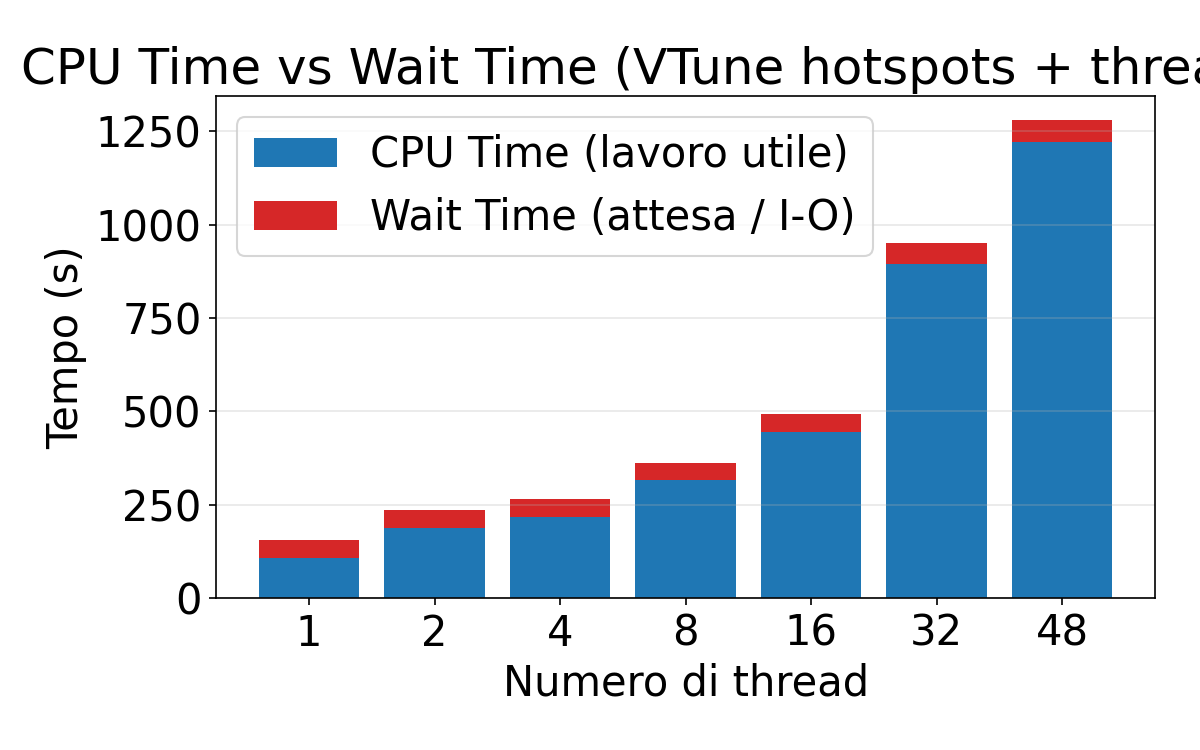
\includegraphics[width=\linewidth]{compute_vs_io_plot.png}
\caption{CPU time (useful computation) vs.\ Wait time (I/O and synchronization) across thread counts, from VTune Hotspots and Threading collections.}
\label{fig:part1-io}
\end{figure}
